\section{Introduction}
\subsection{Uncore Intellectual Properties}
Intel System on a Chip (SoC) features a new set of Intel Uncore Intellectual Property (IP)
for every generation. The Uncore encompasses system agent (SA), memory and Uncore agents
such as graphics controller, display controller, memory controller and Input Output (IO). The
Uncore IPs are Peripheral Component Interface Express (PCIe), Graphics Processing Engine
(GPE), Thunderbolt, Imaging Processing Agent (IPU), North Peak (NPK), Virtualization
Technology for directed-IO (Vt-d), Volume Management Device (VMD).

PCI Express abbreviated as PCIe or PCI-E, is designed to replace the older PCI standards.
A data communication system is developed for use the transfer data between the host and the
peripheral devices via PCIe. Thunderbolt is the brand name of a hardware interface developed
by Intel that allows the connection of external peripherals to a computer. Thunderbolt combines
PCI Express (PCIe) and DisplayPort (DP) into two serial signals, and additionally provides DC
power, all in one cable. Graphics Processing Engine (GPE), Integrated graphics, shared graphics
solutions, integrated graphics processors (IGP) or unified memory architecture (UMA) utilize a
portion of a computer's system RAM rather than dedicated graphics memory. GPEs can be
integrated onto the motherboard as part of the chipset. Virtual Technology for Directed-IO (Vt-d)
is an input/output memory management unit (IOMMU) allows guest virtual machines to directly
use peripheral devices, such as Ethernet, accelerated graphics cards, and hard-drive controllers,
through DMA and interrupt remapping.

\subsection{Legacy \gls{bios} and \gls{uefi}}

\paragraph{\gls{bios}} is the dominant standard which defines a firmware interface.

"Legacy" (as in Legacy \gls{bios}), in the context of firmware specifications, refer to an older, widely used specification. Major responsibility of \gls{bios} is to set up the hardware, load and start an \gls{os}. When the system boots, the BIOS initializes and identifies system devices including video display card, mouse, hard disk drive, keyboard, solid state drive and other hardware followed by locating software held on a boot device i.e. a hard disk or removable storage such as CD/DVD or USB and loads and executes that software, giving it control of the computer. This process is also referred to as "booting" or "boot strapping".

\subsubsection{Background of Legacy \gls{bios}}
In 1980s, IBM developed the personal computer with a 16-bit BIOS with the aim of ending the BIOS after the first 250,000 products. Legacy BIOS is based upon Intel's original 16-bit architecture, ordinarily referred to as  "8086" architecture. And as technology advanced, Intel extended that 8086 architecture from 16 to 32-bit.
Legacy BIOS is able to run different \gls{os}, such as MS-DOS, equally well on systems other than IBM. Additionally, Legacy BIOS has a defined OS-independent interface for hardware that enables interrupts to communicate with video, disk and keyboard services along with the BIOS ROM loader and bootstrap loader, to name a few.

Use of legacy BIOS is diminishing and is expected to be phased out in new systems by the year 2020.

\subsubsection{Limitations of legacy BIOS}
Over the years, many new configuration and power management technologies were integrated
into BIOS implementations as well as support for many generations of Intel® architecture
hardware. However certain limitations of BIOS implementations such as 16-bit addressing mode,
1 MB addressable space, PC AT hardware dependencies and upper memory block (UMB)
dependencies persisted throughout the years. The industry also began to have need for methods to
ensure quality of individual firmware modules as well as the ability to quickly integrate libraries
of third-party firmware modules into a single platform solution across multiple product lines.
These inherent limitations and existing market demands opened the opportunity for a fresh BIOS
architecture to be developed and introduced to the market. The UEFI specifications and resulting
implementations have begun to effectively address these persisting market needs.

One of the critical maintenance challenges for BIOS is that each implementation has tended to
be highly customized for the specific motherboard on which it is deployed. Moving component
modules across designs typically requires significant porting, integration, testing and debug work.
This is one of the markets challenges the UEFI architecture promises to address.

\subsection{Unified Extensible Firmware Interface (\gls{uefi})}
\gls{uefi} was developed as a replacement for legacy BIOS to streamline the booting process, and act as the interface between a operating system and its platform firmware. It not only replaces most BIOS functions, but also offers a rich extensible pre-OS environment with advanced boot and runtime services.
Unified Extensible Firmware Interface (\gls{uefi}) is grounded in Intel's initial Extensible Firmware Interface (EFI) specification 1.10, which defines a software interface between an operating system and platform firmware. The UEFI architecture allows users to execute applications on a command line interface. It has intrinsic networking capabilities and is designed to work with multi-processors (MP) systems.

\begin{figure}[h]
	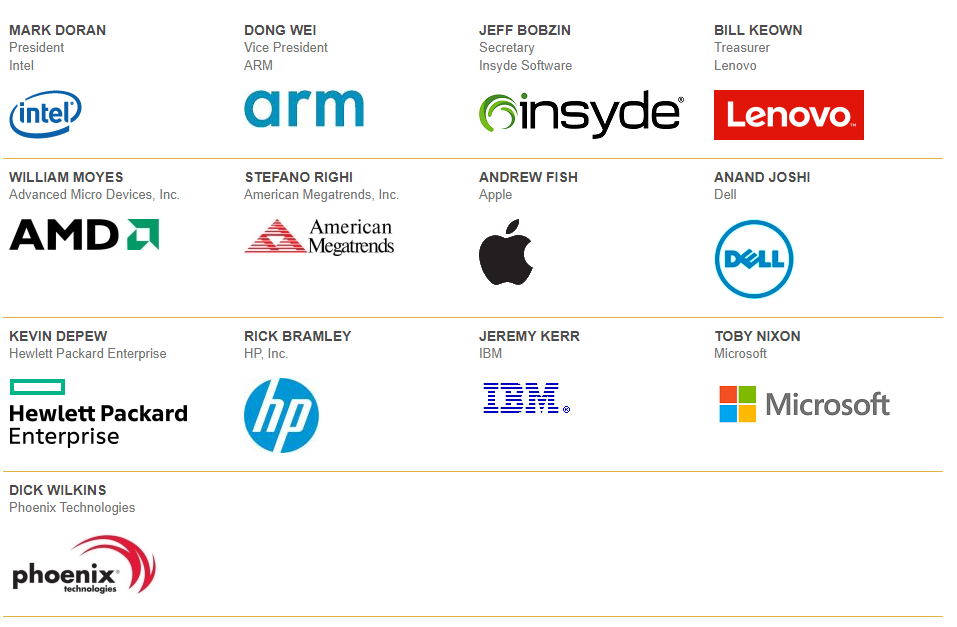
\includegraphics[width=\linewidth]{uefi_board_of_directors}
	\caption{Board of Directors of UEFI Forum}\label{fig:introduction-uefi-board-of-directors}
\end{figure}

The UEFI Forum board of directors consists of representatives from 11 industry leaders as described in Figure \ref{fig:introduction-uefi-board-of-directors}. These involved organizations work to ensure that the UEFI specifications meet industry needs.

UEFI uses a different interface for boot services and runtime services but UEFI does not specify how "Power On Self Test" (POST) and Setup are implemented - those are BIOS' primary functions.

\subsubsection{\gls{uefi} Driver Model Extension}
Access to boot devices is provided through a set of protocol interfaces. One purpose of the
UEFI Driver Model is to provide a replacement for \verb|PC-AT|-style option ROMs. It is important
to point out that drivers written to the UEFI Driver Model are designed to access boot devices in
the pre-boot environment. They are not designed to replace the high-performance, OS-specific
drivers.

The UEFI Driver Model is designed to support the execution of modular pieces of code,
also known as drivers, that run in the pre-boot environment. These drivers may manage or control
hardware buses and devices on the platform, or they may provide some software-derived, platform specific service. The UEFI Driver Model also contains information required by UEFI driver writers to design and implement any combination of bus drivers and device drivers that a platform
might need to boot a UEFI-compliant OS.

The UEFI Driver Model is designed to be generic and can be adapted to any type of bus or
device. The UEFI Specification describes how to write PCI bus drivers, PCI device drivers, USB
bus drivers, USB device drivers, and SCSI drivers. Additional details are provided that allow UEFI
drivers to be stored in PCI option ROMs, while maintaining compatibility with legacy option ROM
images.

One of the design goals in the UEFI Specification is keeping the driver images as small as
possible. However, if a driver is required to support multiple processor architectures, a driver
object file would also be required to be shipped for each supported processor architecture. To
address this space issue, this specification also defines the EFI Byte Code Virtual Machine. A
UEFI driver can be compiled into a single EFI Byte Code object file. UEFI Specificationcomplaint firmware must contain an EFI Byte Code interpreter. This allows a single EFI Byte
Code object file that supports multiple processor architectures to be shipped. Another space saving
technique is the use of compression. This specification defines compression and decompression
algorithms that may be used to reduce the size of UEFI Drivers, and thus reduce the overhead
when UEFI Drivers are stored in ROM devices.

The information contained in the UEFI Specification can be used by OSVs, IHVs, OEMs,
and firmware vendors to design and implement firmware conforming to this specification, drivers
that produce standard protocol interfaces, and operating system loaders that can be used to boot
UEFI compliant operating systems.

\subsubsection{\gls{uefi}'s Role in boot process}

During the boot process, UEFI speaks to the operating system loader and acts as the interface between the operating system and the BIOS.

The \verb|PC-AT| boot environment presents significant challenges to innovation within the
industry. Each new platform capability or hardware innovation requires firmware developers to
craft increasingly complex solutions, and often requires OS developers to make changes to their
boot code before customers can benefit from the innovation. This can be a time-consuming process
requiring a significant investment of resources. The primary goal of the UEFI specification is to
define an alternative boot environment that can alleviate some of these considerations. In this goal, the specification is like other existing boot specifications.

\subsection{Comparing of Legacy \gls{bios} and \gls{uefi}}

\begin{table}
	\centering
	\renewcommand{\arraystretch}{2}
	\caption{Legacy BIOS v/s UEFI}\label{table:legacy-bios-vs-uefi}
	\begin{tabular}{l | p{5cm} | p{5cm}}
		& Legacy BIOS & EFI
		\\ \hline \hline
		Language & Assembly & C ($ 99\% $)
		\\ \hline
		Resource & Interrupt Hardcode Memory Access hardcore I/O Access & Diver, Protocols
		\\ \hline
		Processor & x86 16-bit & CPU Protects Mode (Flat Mode)
		\\ \hline
		Expand & Hook Interrupt & Load Driver
		\\ \hline
		OS Bridge & ACPI & Run Time Driver Software
		\\ \hline
		$ 3^{rd} $ Party ISV \& IHV & Bas for Support & Easy for Support and for Multi Platforms
		\\ \hline
	\end{tabular}
\end{table}


\subsection{Advanced Configuration and Power Interface (\gls{acpi})}
The ACPI Component Architecture (ACPICA) defines and implements a group of software
components that together create an implementation of the ACPI specification. A major goal of the
architecture is to isolate all operating system dependencies to a relatively small translation or
conversion layer (the OS Services Layer) so that the bulk of the ACPICA code is independent of
any individual operating system. Therefore, hosting the ACPICA code on new operating systems
requires no source changes within the ACPICA code itself.

The components of the architecture include:
\begin{itemize}
	\item An OS-independent, kernel-resident ACPICA Subsystem component that provides the fundamental ACPI services such as the AML interpreter and namespace management.
	\item An OS-dependent OS Services Layer for each host operating system to provide OS support for the OS-independent ACPICA Subsystem.
	\item An ASL compiler-disassembler for translating ASL code to AML byte code and for disassembling existing binary ACPI tables back to ASL source code.
	\item Several ACPI utilities for executing the interpreter in ring 3 user space, extracting binary ACPI tables from the output of the ACPI Dump utility, and translating the ACPICA source	code to Linux/Unix format.
\end{itemize}

In Figure \ref{fig:introduction-acpi-component-architecture}, the ACPICA subsystem is shown in relation to the host operating system, device driver, OSPM software, and the ACPI hardware

\begin{figure}[h]
	\centering
	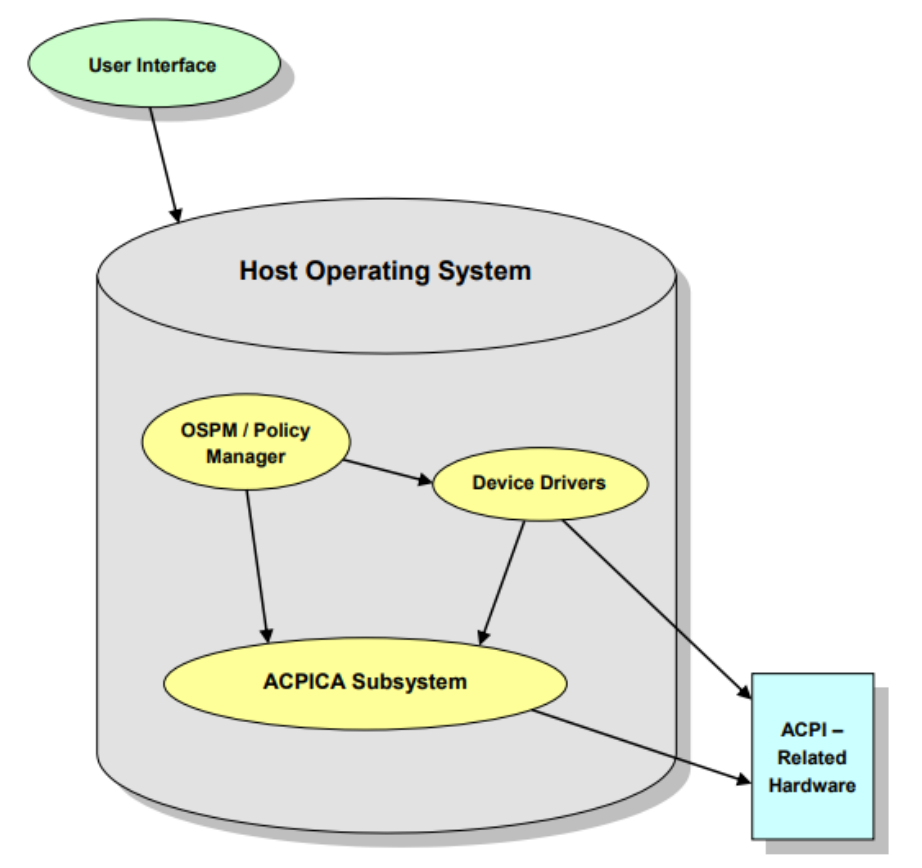
\includegraphics[width=0.7\linewidth]{introduction/acpi-component-architecture}
	\caption{The \gls{acpi} Component Architecture}\label{fig:introduction-acpi-component-architecture}
\end{figure}

\subsubsection{Overview of ACPICA Subsystem}
The ACPICA Subsystem implements the low level or fundamental aspects of the ACPI
specification. Included are an AML parser/interpreter, ACPI namespace management, ACPI table
and device support, and event handling. Since the ACPICA subsystem provides low-level system
services, it also requires low-level operating system services such as memory management,
synchronization, scheduling, and I/O.

To allow the ACPICA Subsystem to easily interface to any operating system that provides such
services, an Operating System Services Layer translates ACPICA-to-OS requests into the system
calls provided by the host operating system. The OS Services Layer is the only component of the
ACPICA that contains code that is specific to a host operating system.

Thus, the ACPICA Subsystem consists of two major software components:
\begin{itemize}
	\item The basic kernel-resident ACPICA Subsystem provides the fundamental ACPI services	that are independent of any particular operating system.
	\item The OS Services Layer (OSL) provides the conversion layer that interfaces the OS independent ACPICA Subsystem to a host operating system.
\end{itemize}

When combined into a single static or loadable software module such as a device driver or
kernel subsystem, these two major components form the ACPICA Subsystem. Throughout this
document, the term "ACPICA Subsystem" refers to the combination of the OS-independent
ACPICA Subsystem with an OS Services Layer components combined into a single module,
driver, or load unit.

\subsubsection{OS-independent ACPICA Subsystem}
The OS-independent ACPICA Subsystem supplies the major building blocks or subcomponents that are required for all ACPI implementations — including an AML interpreter, a namespace manager, ACPI event and resource management, and ACPI hardware support.

One of the goals of the ACPICA Subsystem is to provide an abstraction level high enough such
that the host operating system does not need to understand or know about the very low-level ACPI
details. For example, all AML code is hidden from the host. Also, the details of the ACPI hardware
are abstracted to higher-level software interfaces.

The ACPICA Subsystem implementation makes no assumptions about the host operating system or environment. The only way it can request operating system services is via interfaces provided by the OS Services Layer.

The primary user of the services provided by the ACPICA Subsystem are the host OS device drivers and power/thermal management software.

\subsubsection{Operating System Services Layer}
The OS Services Layer (or OSL) operates as a translation service for requests from the OS independent ACPICA subsystem back to the host OS. The OSL implements a generic set of OS service interfaces by using the primitives available from the host OS. Because of its nature.

The OS Services Layer must be implemented anew for each supported host operating
system. There is a single OS-independent ACPICA Subsystem, but there must be an OS Services
Layer for each operating system supported by the ACPI component architecture.

The primary function of the OSL in the ACPI Component Architecture is to be the small
glue layer that binds the much larger ACPICA Subsystem to the host operating system. Because
of the nature of ACPI itself — such as the requirement for an AML interpreter and management
of a large namespace data structure — most of the implementation of the ACPI specification is
independent of any operating system services. Therefore, the OS-independent ACPICA Subsystem
is the larger of the two components.

The overall ACPI Component Architecture in relation to the host operating system is Figure

\begin{figure}[h]
	\centering
	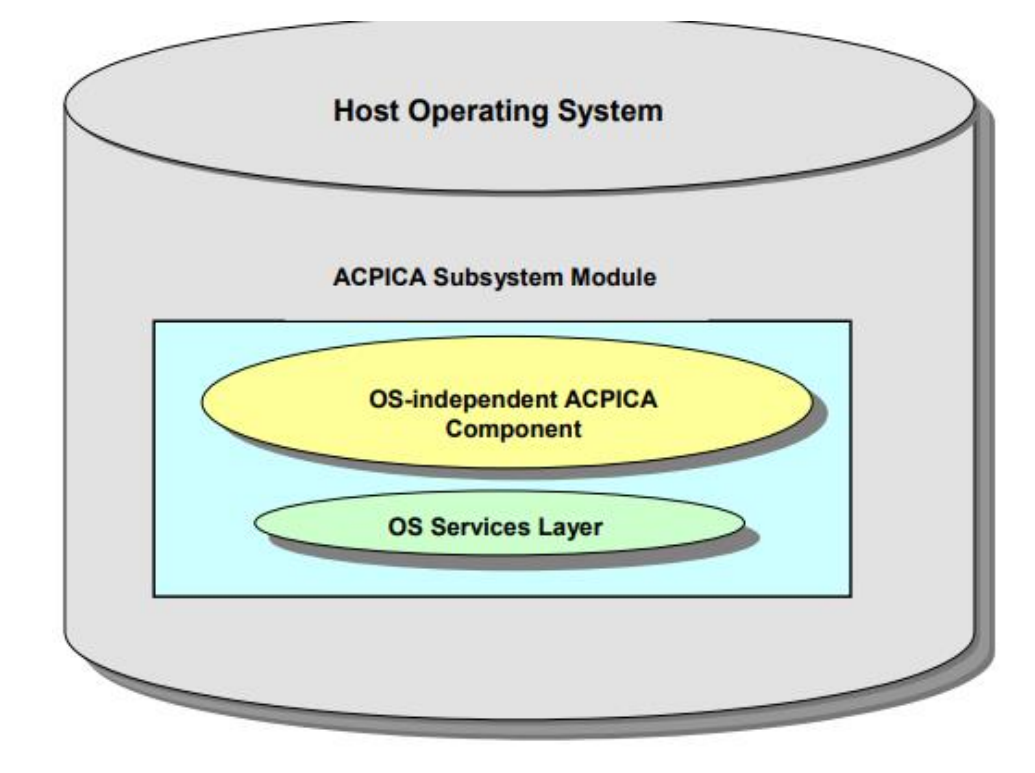
\includegraphics[width=0.7\linewidth]{introduction/acpica-subsystem-architecture}
	\caption{ACPICA Subsystem Architecture}\label{fig:introduction-acpica-subsystem-architecture}
\end{figure}

\subsubsection{ACPICA Subsystem Interaction}
The ACPICA Subsystem implements a set of external interfaces that can be directly called from
the host OS. These Acpi* interfaces provide the actual ACPI services for the host. When operating
system services are required during the servicing of an ACPI request, the Subsystem makes
requests to the host OS indirectly via the fixed AcpiOs* interfaces. The diagram below illustrates
the relationships and interaction between the various architectural elements by showing the flow
of control between them. Note that the OS-independent ACPICA Subsystem never calls the host directly instead it makes calls to the AcpiOs * interfaces in the OSL. This provides the ACPICA
code with OS-independence.

The Interaction between the Architectural Components Is shown in Figure \ref{fig:-introduction-acpi-interaction-between-the-architectural-components}

\begin{figure}[h]
	\centering
	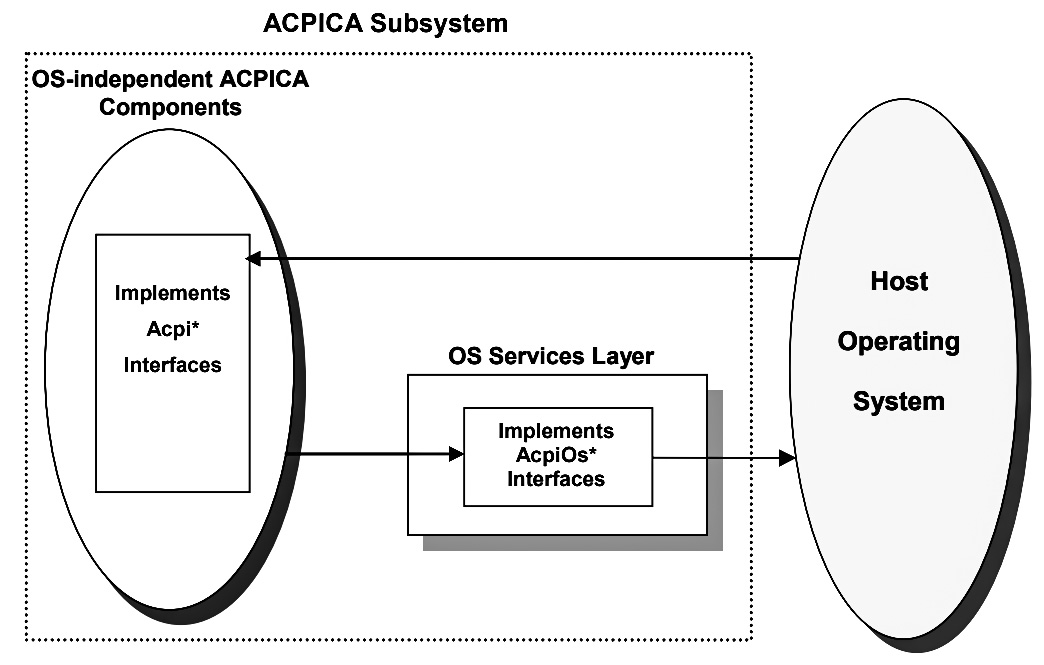
\includegraphics[width=0.7\linewidth]{introduction/acpi-interaction-between-the-architectural-components}
	\caption{Interaction between the Architectural Components}\label{fig:-introduction-acpi-interaction-between-the-architectural-components}
\end{figure}


\subsection{Peripheral Component Interconnect Express (\gls{pcie})}
The \say{Peripheral Component Interconnect (PCI)} architecture has emerged out to be a very thriving beyond even the many more optimistic prospects. Today about every new computer system arrives equipped with at least one PCI slots. Even though there are about to countless PCI slots are shipped globally, there does exists tons of PCI adapter cards which are available to fulfill the all the virtual possible application needs.

This fast growing generation has also raised the demand for many new higher performance interface for input-output communication to support rising technology such as ultra high bandwidth technologies like $ 10-Gb $ Ethernet, $ 10-Gb $ \say{FibreChannel}, $ 12X $ InfiniBand and many more. A regulation which could adapt to carrying out these high performance objectives, while withholding compatibility for previous generation of PCI would beyond any doubt can offer the idealistic solution.

\say{PCI-X 2.0} standard has been developed to meet these objectives. It is capable to serve the uninterrupted performance to feed the nearly all high-bandwidth programs while at the same instance keeping up the full hardware and software backward compatibility for previous \say{PCI} and \say{PCI-X} generations. The PCI-X 2.0 regulation establishes two new grades of speed and performance which are PCI-X 266 and PCI-X 533. These speed grades endeavors bandwidths that are twice and fourfold that of previous generation PCI-X 133 which results to finally supplying bandwidths which are $ 32x $ faster compared to the older version of PCI. It successfully succeeds to bring of additional required performance via time-proven \say{Double Data Rate (DDR)} and \say{Quad Data Rate (QDR)} mechanisms that transmit data at either twice or fourfold the base frequency of clock. As the PCI-X 2.0 conserves too many modules of previous generation PCI it's beneficiary for terrific amount of preceding development job. The OS, device drivers, protocols, connectors, form factor, BIOS, electrical signals, Bus functional modal among many more original PCI modules are all greatly rendered in the new PCI-X 2.0 specification.
Also, many of these modules actually remains untouched in PCI-X 2.0. Due to not having the much of the dissimilarity, it enables development easier because these modules have been already designed and developed with required engineering and familiar to the developers. As a end result, risk is dramatically decreased because the time-to-market became short.

\subsubsection{Functional Description}
The hardware which is used to implement a PCI based system consumes a software interface served by PCI BIOS feature. It has elementary use to generate operations in address spaces specific to PCI (PCI configuration space).

The X86 architecture allows following mode to operate as per PCI BIOS features:
\begin{itemize}
  \item Real mode
  \item Protected mode
    \begin{itemize}
      \item $ 286 $ protected mode $ (16:16) $
      \item $ 386 $ protected mode $ (16:32) $
    \end{itemize}
  \item Flat mode (0:32 protected mode)
\end{itemize}
In the Flat mode, all the segments begun at linear address $ 0 $ and span till the end of the whole $ 4-GB $ address space.

\subsubsection{BUS Performances and Number of Slots Compared}
The several architectures characterized by the PCISIG. Figure \ref{fig:comparison-of-bus-frequency-bandwidth-slots} portrays the development of PCI bus clock frequencies and bandwidths. Its pretty obvious that the increasing the bus frequency does comprise the load in terms of electrical nodes as also to the maximum permissible connectors on a bus at that clock frequencies.

\begin{figure}[!htbp]
	\centering
	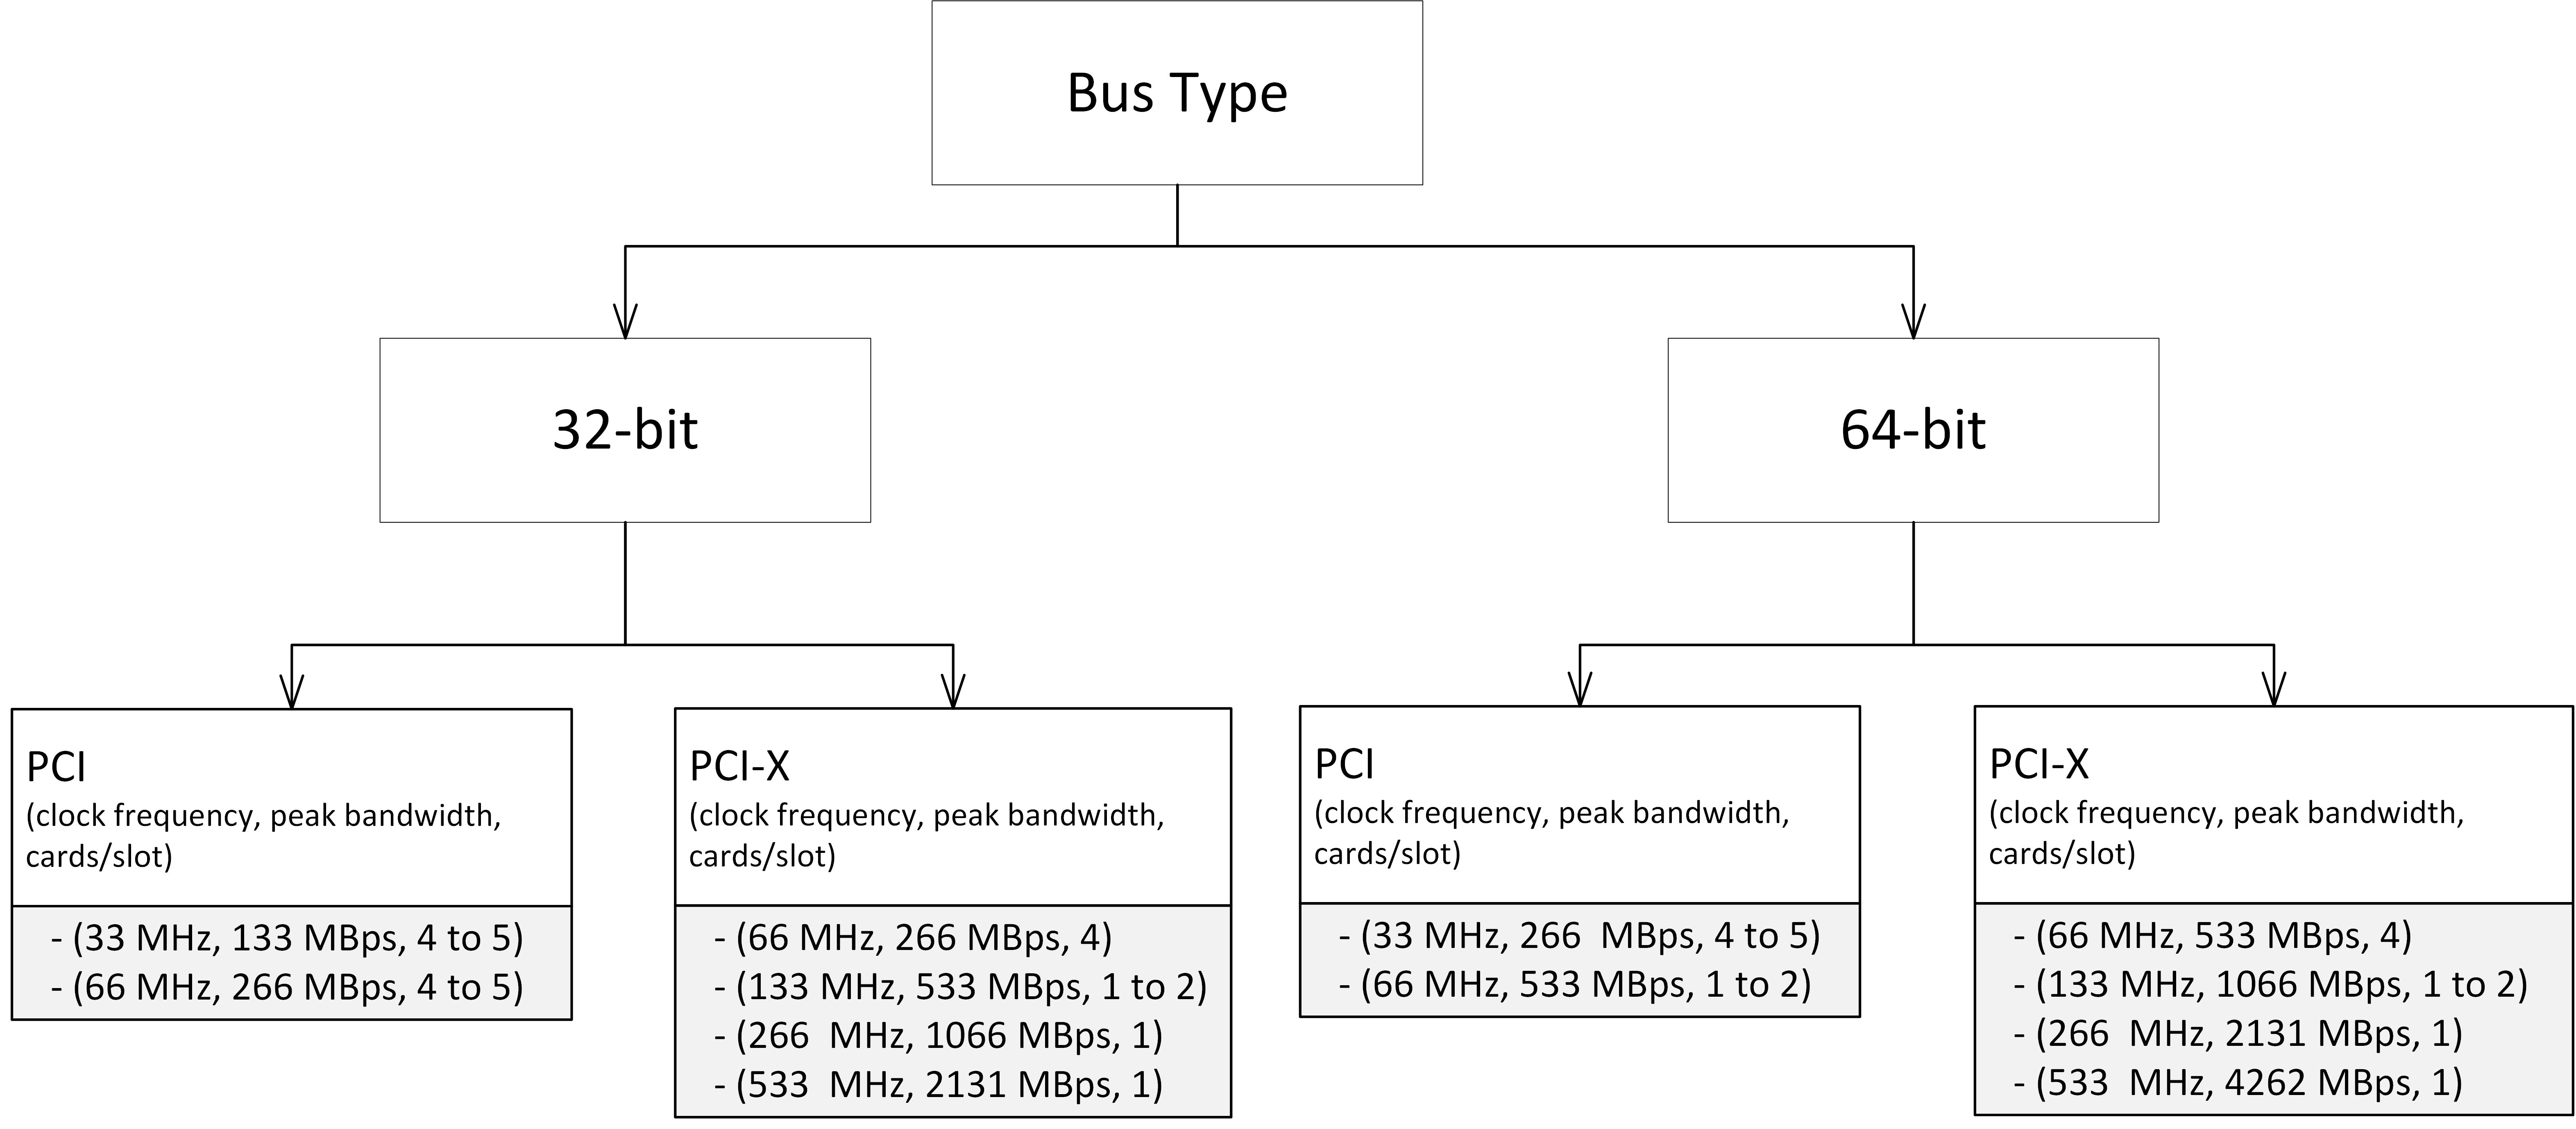
\includegraphics[width=\linewidth]{introduction/comparison-of-bus-frequency-bandwidth-slots}
	\caption{Comparison of Bus Frequency, Bandwidth and Number of Slots}\label{fig:comparison-of-bus-frequency-bandwidth-slots}
\end{figure}

A \say{PCI express (PCIe) Interconnect} is responsible in connecting two PCI devices via PCI link. A PCI link consists if any signal pairs in each direction. These signals ($ x1, x2, x4, x8, x12, x16, x32 $) known as the Lanes. A BIOS designer decides that how many Lanes implementation should be permissible based on the benchmark performance of targeted platform on a given PCI link.

Figure \ref{fig:comparison-of-bus-frequency-bandwidth-slots} portrays the total bandwidth values for various PCI link width.



\subsection{Graphics Controller}
Almost every graphics controllers are merely PCI controllers only. And it is also obvious that the graphics drivers who are responsible to control and manage these graphics controllers are also PCI drivers. Note that even if the most graphics controllers are PCI controllers but even then the graphics controllers can also utilize many of the other buses i.e. USB buses. 

Characterizes of Graphics drivers are listed below:
\begin{itemize}
	\item Follows UEFI Driver Modal
	\item Depending on the driver manged adapter, a graphics driver could be classified as into: a single output adapter and a multiple output adapter.
	\item For each output expected, the graphics driver has to construct child handles.
	\item For some of the output ports and protocols (such as GOP Protocol) the graphics drivers must create child handles.
	\item Graphics drivers are chip-specific because of the requirement to initialize and manage the graphics device.
\end{itemize}
Note that (\gls{ihv}) has privilege for choosing whether to support and implement all the required modules of the UEFI specification. i.e., all modules might not be implemented to support on a specified system configuration which doesn't support all of the services and features understood by the needed modules.

\subsubsection{Graphics Output Protocol (\gls{gop})}
The \say{Graphics Output Protocol \gls{gop}} Driver is member of the driver of UEFI boot time which are responsible for running up the display while the bios is booting. This driver triggers displaying of logo while the bios is booting.

\subsubsection{GOP Overview}
The GOP driver is the successor for video controller of legacy BIOS and sheers the utilization of UEFI pre-boot firmware without the use of CSM. The GOP driver can be $ 32-bit $, $ 64-bit $, or $ IA-64 $ with no binary support. Pre-boot firmware architecture of UEFI which could be either $ 32-bit $ or $ 64-bit $ has to adapt the corresponding GOP driver architecture ($ 32-bit $ or $ 64-bit $). The GOP driver could be one of the boot mode: \say{fastboot} (for specific platform optimized mode to speedup the boot time) or \say{generic} (the normal boot process).

\subsubsection{GOP DRIVER}
The EFI specification characterizes the \say{Universal Graphic Adapter (UGA)} protocol to provide graphics which could be device-independent. However, Specification of UEFI eliminated the inclusion of UGA and replaced it with it's successor \gls{gop} so that VGA hardware dependencies can be removed.

\subsubsection{GOP Integration}
The platform firmware must meet the following requirements for GOP Driver integration:
\begin{itemize}
	\item Platform firmware must be compliant to UEFI 2.1 or later.
	\item Platform must enumerate and initialize the graphics device.
	\item Platform must allocate enough graphics frame buffer memory required to support the native mode resolution of the integrated display.
	\item The platform must produce the standard \verb|EFI_PCI_IO_PROTOCOL| and as well as the \verb|EFI_DEVICE_PATH_PROTOCOL| on the graphics device handle. Additionally, the platform must produce \verb|PLATFORM_GOP_POLICY_PROTOCOL|.
	\item The platform firmware must not launch the legacy Video BIOS.
\end{itemize}

The GOP Driver solution comprises the following files shown in Table \ref{table:gop-driver-files} GOP driver files.

\begin{table}
	\centering
	\renewcommand\arraystretch{2}
	\caption{\gls{gop} Driver files}\label{table:gop-driver-files}
	\begin{tabular}{l | p{5cm} | p{5cm}}
		File Name & Description & Format
		\\ \hline \hline
		\verb|GopDriver.efi| & The \gls{gop} driver binary & Uncompressed PE/COFF image
		\\ \hline
		\verb|Vbt.bin| & Contains Video BIOS Table (VBT) data & Raw Binary
		\\ \hline
		\verb|Vbt.bsf| & BMP script file. Required for modifying Vbt.bin using BMP tool & Text
		\\ \hline
	\end{tabular}
\end{table}

Customize the VBT data file\verb| Vbt.bin| as per platform requirements and the corresponding BSF file. Integrate \verb|Vbt.bin| and \verb|GopDriver.efi| files into the platform firmware image. The process of accomplishing this step is determined by the platform implementer, specific to the platform firmware implementation.

